\documentclass{article}
\usepackage[utf8]{inputenc}

\usepackage{fancyhdr}
\usepackage{hyperref}

\usepackage[a4paper, total={6in, 8in}]{geometry}
\usepackage{amsfonts}
\usepackage{amsmath}
\usepackage{amsthm}
\DeclareMathOperator{\Sym}{Sym}

\usepackage{tikz}

\usepackage{graphicx}

\newtheorem{theorem}{Theorem}[section]
\newtheorem{corollary}{Corollary}[theorem]
\newtheorem{definition}{Definition}[section]

\title{2D Rubik's Shapes and the the analysis of good 2D Rubik's Shapes sharing one side \textbf{[Not clear]}}
\author{Logan Crone, Andy Dilks, Lior Fishman, Brandon Mather, Skylar Werner\\
University of North Texas *}
\date{Date}

\begin{document}

\maketitle
\begin{abstract}
    The Rubik's cube was invented in 1974 by Erno Rubik, who had no idea of the incredible popularity and mathematical fascinations his toy would bring. Through the years of study on how the cube operates, the Rubik's Group was formed to represent all possible moves one could perform on the cube. In this paper, we define a planar analogue to the Rubik's cube, aptly dubbed the Rubik's Square, and prove that the Rubik's square is \textit{good}. We then abstractive the Rubik's Square to a Rubik's Shape and analyse the \textit{goodness} of the subcase where the sides shared is of length one.
\end{abstract}

\textbf{[Put at the bottom of Page 1 $\backslash/$]}

\noindent\rule{6cm}{0.4pt}

*Address:\;\; Department of Mathematics, University of North Texas, 1155 Union Circle \# 311430, Denton TX, 76203-5017, USA; E-mail:\;\; \href{mailto:lcronest@gmail.com}{lcronest@gmail.com}, \href{mailto:jeremydilks@my.unt.edu}{jeremydilks@my.unt.edu}, \href{mailto:brandonmather@my.unt.edu}{brandonmather@my.unt.edu}, \href{mailto:lior.fishman@unt.edu}{lior.fishman@unt.edu}, \href{mailto:skylar\_werner@yahoo.com}{skylar\_werner@yahoo.com}

\section{Background: Rubik's cube}

\section{$2\times 2$ Rubik's square}

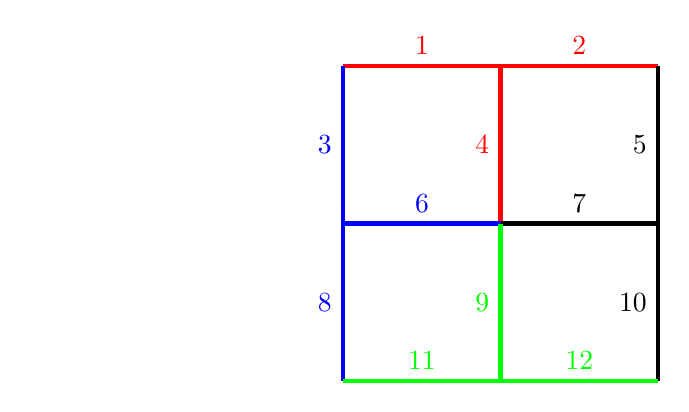
\begin{tikzpicture}
    \draw[white] (0,0) -- (8,0);
    \draw[red, ultra thick] (4,2) -- node[above] {1} (6,2);
    \draw[red, ultra thick] (6,2) -- node[above] {2} (8,2);
    \draw[red, ultra thick] (6,2) -- node[left] {4} (6,0);
    \draw[blue, ultra thick] (4,2) -- node[left] {3} (4,0);
    \draw[blue, ultra thick] (4,0) -- node[left] {8} (4,-2);
    \draw[blue, ultra thick] (4,0) -- node[above] {6} (6,0);
    \draw[black, ultra thick] (8,2) -- node[left] {5} (8,0);
    \draw[black, ultra thick] (8,0) -- node[left] {10} (8,-2);
    \draw[black, ultra thick] (6,0) -- node[above] {7} (8,0);
    \draw[green, ultra thick] (4,-2) -- node[above] {11}(6,-2);
    \draw[green, ultra thick] (6,-2) -- node[left] {9}(6,0);
    \draw[green, ultra thick] (6,-2) -- node[above] {12}(8,-2);
\end{tikzpicture}

\begin{itemize}
    \item $M_1 = (1\,4\,6\,3)$
    \item $M_2 = (2\,5\,7\,4)$
    \item $M_3 = (6\,9\,11\,8)$
    \item $M_4 = (7\,10\,12\,9)$
\end{itemize}

\textbf{$2\times 2$ Square Permutations}: $\frac{12!}{4 \times 3!} = 1.9958\times10^7$.

\textbf{Color Group Moves}: Show def and then show them.

\textbf{Line Moves:} Show def and then show them.

\textbf{Blurb about how this solves any possible state.}

\textbf{Algebraic Model:} $\left<M_1, M_2, M_3, M_4\right> \cong S_{12}$

\textbf{Conjecture:} The $n \times n$ Rubik's Square is isomorphic to $S_{2n(n+1)}$, where $2n(n+1)$ is the number of lines on the square.

\textbf{$3 \times 3$ and $5 \times 5$ Rubik's Square:} Show as an example and then talk about when $n$ is odd and thus can't be constructed out of other squares which is big sad.

\section{Questions about Rubik's square}

\textbf{Efficient algorithm}

\textbf{God's Number}

\textbf{Algebraic Model for Rubik's square}

\textbf{Algorithm}

\section{2D Rubik's shape with one connected edge given one shape has an even side}

\begin{definition}
    A \emph{2d-Rubik's shape} is a graph $G$, with a set of distinguished cycles $\{C_1, \dots, C_n\}$ of $G$  which is built up by induction as follows:

    \begin{enumerate}
        \item The $n$-cycles for $n \geq 3$ are all 2d-Rubik's shapes.
        \item Given a 2d-Rubik's shape $G$ with distinguished cycles $\{C_1, \dots C_n\}$, if we let $P$ be a path in $G$ with at least two vertices so that $E(P) \cap E(C_i) \cap E(C_j) = \emptyset$ for any distinct $i, j$, and let $G' = G \cup \{v_1, \dots v_k\}$ with $v_i E' v_{i+1}$ and $v_1$ is connected to one endpoint of $P$ by an edge, and $v_k$ is connected to the other endpoint of $P$, then $G'$, together with the distinguished cycles $\{C_1, \dots C_n\} \cup \{P \cup \{v_1, \dots v_k\}\}$ is a 2d-Rubik's shape.\\

              Given a 2d-Rubik's shape $G$ with distinguished cycles $\{C_1, \dots C_n\}$, if we let $P$ be a path in $G$ with at least two vertices so that $E(P) \subset E(C_i)$ for some $i$, and let $G' = G \cup \{v_1, \dots v_k\}$ with $v_i E' v_{i+1}$ and $v_1$ is connected to one endpoint of $P$ by an edge, and $v_k$ is connected to the other endpoint of $P$, then $G'$, together with the distinguished cycles $\{C_1, \dots C_n\} \cup \{P \cup \{v_1, \dots v_k\}\}$ is a 2d-Rubik's shape.
    \end{enumerate}
\end{definition}

\begin{definition}
    A 2d-Rubik's shape $G, \{C_1, \dots C_n\}$ is \emph{good} if the subgroup of $H \leq \Sym(E(G))$ generated by the permutations $\sigma_1, \dots, \sigma_n$ which respectively rotate the edges of the cycles $C_1, \dots, C_n$ is equal to $\Sym(E(G))$.
\end{definition}
The intuition behind this definition is that a good 2d-Rubik's shape can be returned by use of the allowed permutations $\sigma_1, \dots \sigma_n$ from any initial configuration of the edges to the starting configuration.

\begin{theorem}
    Suppose that $G$ is a 2d-Rubik's shape with distinguished cycles ${C_1, C_2}$ and that the length of at least one of $C_1, C_2$ is even and $|E(C_1) \cap E(C_2)| = 1$.  Then $G$ is a good 2d-Rubik's shape.
\end{theorem}
\begin{proof}
    Suppose without loss of generality that $\sigma_1$ has even order.
    Label the edges of $C_1$ by $(0, 1, \dots, k)$ and the edges of $C_2$ by $(0, k+\ell, k+\ell-1, \dots, k+2, k+1)$, so that if we identify $\sigma_1, \sigma_2$ with the corresponding elements of $\Sym(k+\ell+1)$ then $\sigma_1$ is the cycle $(0, 1, \dots, k)$ and $\sigma_2$ is the cycle $(0, k+\ell, k+\ell-1, \dots, k+2, k+1)$

    We claim that if $0\leq j-1 < j \leq k$ then the product,
    \[ \sigma_1^{j+1}\left(\sigma_2^{-1}\sigma_1\sigma_2\sigma_1\right)^{\frac{k-2}{2}}\sigma_2^{-1}\sigma_1^2\sigma_2\sigma_1^{k+1-j} \]
    will transpose the edges $j-1$ and $j$.

    \tikzset{every picture/.style={line width=0.75pt}} %set default line width to 0.75pt        

    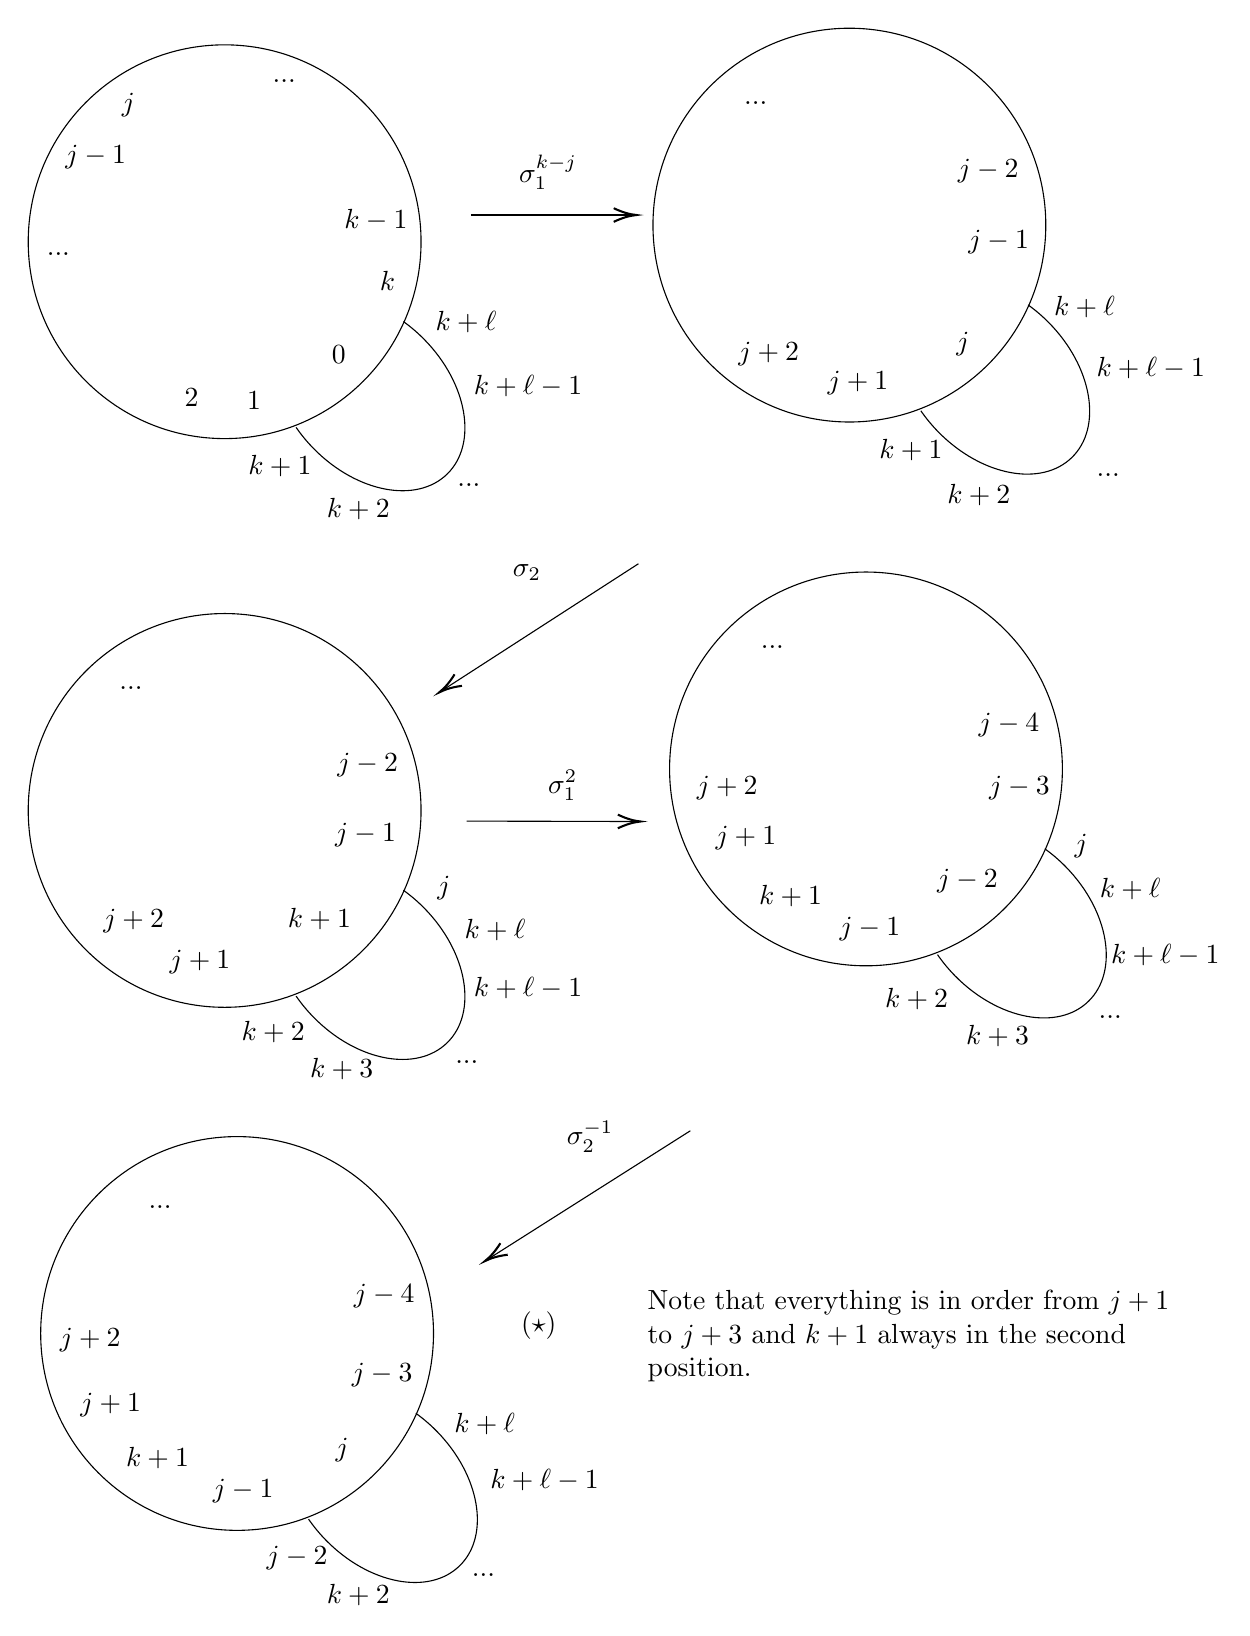
\begin{tikzpicture}[x=0.75pt,y=0.75pt,yscale=-1,xscale=1]
        %uncomment if require: \path (0,789); %set diagram left start at 0, and has height of 789

        %Shape: Ellipse [id:dp3851473480685037] 
        \draw   (22.79,105.86) .. controls (22.79,53.47) and (65.16,11) .. (117.42,11) .. controls (169.69,11) and (212.05,53.47) .. (212.05,105.86) .. controls (212.05,158.25) and (169.69,200.72) .. (117.42,200.72) .. controls (65.16,200.72) and (22.79,158.25) .. (22.79,105.86) -- cycle ;
        %Shape: Arc [id:dp26747108016752974] 
        \draw  [draw opacity=0] (203.55,144.32) .. controls (207.03,146.82) and (210.42,149.7) .. (213.61,152.95) .. controls (234.47,174.19) and (239.44,203.18) .. (224.73,217.7) .. controls (210.01,232.23) and (181.17,226.78) .. (160.31,205.54) .. controls (157.12,202.29) and (154.3,198.86) .. (151.86,195.32) -- (186.96,179.25) -- cycle ; \draw   (203.55,144.32) .. controls (207.03,146.82) and (210.42,149.7) .. (213.61,152.95) .. controls (234.47,174.19) and (239.44,203.18) .. (224.73,217.7) .. controls (210.01,232.23) and (181.17,226.78) .. (160.31,205.54) .. controls (157.12,202.29) and (154.3,198.86) .. (151.86,195.32) ;
        %Shape: Ellipse [id:dp048293129611794106] 
        \draw   (323.79,97.86) .. controls (323.79,45.47) and (366.16,3) .. (418.42,3) .. controls (470.69,3) and (513.05,45.47) .. (513.05,97.86) .. controls (513.05,150.25) and (470.69,192.72) .. (418.42,192.72) .. controls (366.16,192.72) and (323.79,150.25) .. (323.79,97.86) -- cycle ;
        %Shape: Arc [id:dp7733961558898084] 
        \draw  [draw opacity=0] (504.55,136.32) .. controls (508.03,138.82) and (511.42,141.7) .. (514.61,144.95) .. controls (535.47,166.19) and (540.44,195.18) .. (525.73,209.7) .. controls (511.01,224.23) and (482.17,218.78) .. (461.31,197.54) .. controls (458.12,194.29) and (455.3,190.86) .. (452.86,187.32) -- (487.96,171.25) -- cycle ; \draw   (504.55,136.32) .. controls (508.03,138.82) and (511.42,141.7) .. (514.61,144.95) .. controls (535.47,166.19) and (540.44,195.18) .. (525.73,209.7) .. controls (511.01,224.23) and (482.17,218.78) .. (461.31,197.54) .. controls (458.12,194.29) and (455.3,190.86) .. (452.86,187.32) ;
        %Straight Lines [id:da6645381549538105] 
        \draw    (236,93) -- (313.8,93) ;
        \draw [shift={(315.8,93)}, rotate = 180] [color={rgb, 255:red, 0; green, 0; blue, 0 }  ][line width=0.75]    (10.93,-3.29) .. controls (6.95,-1.4) and (3.31,-0.3) .. (0,0) .. controls (3.31,0.3) and (6.95,1.4) .. (10.93,3.29)   ;
        %Shape: Ellipse [id:dp28346841808278733] 
        \draw   (22.79,379.86) .. controls (22.79,327.47) and (65.16,285) .. (117.42,285) .. controls (169.69,285) and (212.05,327.47) .. (212.05,379.86) .. controls (212.05,432.25) and (169.69,474.72) .. (117.42,474.72) .. controls (65.16,474.72) and (22.79,432.25) .. (22.79,379.86) -- cycle ;
        %Shape: Arc [id:dp5467802088144775] 
        \draw  [draw opacity=0] (203.55,418.32) .. controls (207.03,420.82) and (210.42,423.7) .. (213.61,426.95) .. controls (234.47,448.19) and (239.44,477.18) .. (224.73,491.7) .. controls (210.01,506.23) and (181.17,500.78) .. (160.31,479.54) .. controls (157.12,476.29) and (154.3,472.86) .. (151.86,469.32) -- (186.96,453.25) -- cycle ; \draw   (203.55,418.32) .. controls (207.03,420.82) and (210.42,423.7) .. (213.61,426.95) .. controls (234.47,448.19) and (239.44,477.18) .. (224.73,491.7) .. controls (210.01,506.23) and (181.17,500.78) .. (160.31,479.54) .. controls (157.12,476.29) and (154.3,472.86) .. (151.86,469.32) ;
        %Straight Lines [id:da2550847089224184] 
        \draw    (316.8,261) -- (222.48,321.91) ;
        \draw [shift={(220.8,323)}, rotate = 327.14] [color={rgb, 255:red, 0; green, 0; blue, 0 }  ][line width=0.75]    (10.93,-3.29) .. controls (6.95,-1.4) and (3.31,-0.3) .. (0,0) .. controls (3.31,0.3) and (6.95,1.4) .. (10.93,3.29)   ;
        %Shape: Ellipse [id:dp8651156930485036] 
        \draw   (331.79,359.86) .. controls (331.79,307.47) and (374.16,265) .. (426.42,265) .. controls (478.69,265) and (521.05,307.47) .. (521.05,359.86) .. controls (521.05,412.25) and (478.69,454.72) .. (426.42,454.72) .. controls (374.16,454.72) and (331.79,412.25) .. (331.79,359.86) -- cycle ;
        %Shape: Arc [id:dp4575747283593845] 
        \draw  [draw opacity=0] (512.55,398.32) .. controls (516.03,400.82) and (519.42,403.7) .. (522.61,406.95) .. controls (543.47,428.19) and (548.44,457.18) .. (533.73,471.7) .. controls (519.01,486.23) and (490.17,480.78) .. (469.31,459.54) .. controls (466.12,456.29) and (463.3,452.86) .. (460.86,449.32) -- (495.96,433.25) -- cycle ; \draw   (512.55,398.32) .. controls (516.03,400.82) and (519.42,403.7) .. (522.61,406.95) .. controls (543.47,428.19) and (548.44,457.18) .. (533.73,471.7) .. controls (519.01,486.23) and (490.17,480.78) .. (469.31,459.54) .. controls (466.12,456.29) and (463.3,452.86) .. (460.86,449.32) ;
        %Straight Lines [id:da9619731386949268] 
        \draw    (234,385) -- (315.8,385.2) ;
        \draw [shift={(317.8,385.2)}, rotate = 180.14] [color={rgb, 255:red, 0; green, 0; blue, 0 }  ][line width=0.75]    (10.93,-3.29) .. controls (6.95,-1.4) and (3.31,-0.3) .. (0,0) .. controls (3.31,0.3) and (6.95,1.4) .. (10.93,3.29)   ;
        %Shape: Ellipse [id:dp5569398050814263] 
        \draw   (28.79,631.86) .. controls (28.79,579.47) and (71.16,537) .. (123.42,537) .. controls (175.69,537) and (218.05,579.47) .. (218.05,631.86) .. controls (218.05,684.25) and (175.69,726.72) .. (123.42,726.72) .. controls (71.16,726.72) and (28.79,684.25) .. (28.79,631.86) -- cycle ;
        %Shape: Arc [id:dp7522127717600136] 
        \draw  [draw opacity=0] (209.55,670.32) .. controls (213.03,672.82) and (216.42,675.7) .. (219.61,678.95) .. controls (240.47,700.19) and (245.44,729.18) .. (230.73,743.7) .. controls (216.01,758.23) and (187.17,752.78) .. (166.31,731.54) .. controls (163.12,728.29) and (160.3,724.86) .. (157.86,721.32) -- (192.96,705.25) -- cycle ; \draw   (209.55,670.32) .. controls (213.03,672.82) and (216.42,675.7) .. (219.61,678.95) .. controls (240.47,700.19) and (245.44,729.18) .. (230.73,743.7) .. controls (216.01,758.23) and (187.17,752.78) .. (166.31,731.54) .. controls (163.12,728.29) and (160.3,724.86) .. (157.86,721.32) ;
        %Straight Lines [id:da36554158474057674] 
        \draw    (341.8,534.2) -- (244.49,595.93) ;
        \draw [shift={(242.8,597)}, rotate = 327.61] [color={rgb, 255:red, 0; green, 0; blue, 0 }  ][line width=0.75]    (10.93,-3.29) .. controls (6.95,-1.4) and (3.31,-0.3) .. (0,0) .. controls (3.31,0.3) and (6.95,1.4) .. (10.93,3.29)   ;

        % Text Node
        \draw (167.83,154.82) node [anchor=north west][inner sep=0.75pt]   [align=left] {$\displaystyle 0$};
        % Text Node
        \draw (126.94,176.89) node [anchor=north west][inner sep=0.75pt]   [align=left] {$\displaystyle 1$};
        % Text Node
        \draw (96.82,175.28) node [anchor=north west][inner sep=0.75pt]   [align=left] {$\displaystyle 2$};
        % Text Node
        \draw (30.49,110.01) node [anchor=north west][inner sep=0.75pt]   [align=left] {...};
        % Text Node
        \draw (39.43,57.89) node [anchor=north west][inner sep=0.75pt]   [align=left] {$\displaystyle j-1$};
        % Text Node
        \draw (66.68,33.18) node [anchor=north west][inner sep=0.75pt]   [align=left] {$\displaystyle j$};
        % Text Node
        \draw (139.33,26.62) node [anchor=north west][inner sep=0.75pt]   [align=left] {...};
        % Text Node
        \draw (173.87,88.81) node [anchor=north west][inner sep=0.75pt]   [align=left] {$\displaystyle k-1$};
        % Text Node
        \draw (190.95,118.82) node [anchor=north west][inner sep=0.75pt]   [align=left] {$\displaystyle k$};
        % Text Node
        \draw (127.65,207.65) node [anchor=north west][inner sep=0.75pt]   [align=left] {$\displaystyle k+1$};
        % Text Node
        \draw (165.36,228.25) node [anchor=north west][inner sep=0.75pt]   [align=left] {$\displaystyle k+2$};
        % Text Node
        \draw (236.24,169.13) node [anchor=north west][inner sep=0.75pt]   [align=left] {$\displaystyle k+\ell -1$};
        % Text Node
        \draw (228.28,221.33) node [anchor=north west][inner sep=0.75pt]   [align=left] {...};
        % Text Node
        \draw (217.82,138.11) node [anchor=north west][inner sep=0.75pt]   [align=left] {$\displaystyle k+\ell $};
        % Text Node
        \draw (431.65,199.65) node [anchor=north west][inner sep=0.75pt]   [align=left] {$\displaystyle k+1$};
        % Text Node
        \draw (464.36,221.25) node [anchor=north west][inner sep=0.75pt]   [align=left] {$\displaystyle k+2$};
        % Text Node
        \draw (536.24,160.13) node [anchor=north west][inner sep=0.75pt]   [align=left] {$\displaystyle k+\ell -1$};
        % Text Node
        \draw (536.28,216.33) node [anchor=north west][inner sep=0.75pt]   [align=left] {...};
        % Text Node
        \draw (515.82,131.11) node [anchor=north west][inner sep=0.75pt]   [align=left] {$\displaystyle k+\ell $};
        % Text Node
        \draw (258,63) node [anchor=north west][inner sep=0.75pt]   [align=left] {$\displaystyle \sigma _{1}^{k-j}$};
        % Text Node
        \draw (468.68,148.18) node [anchor=north west][inner sep=0.75pt]   [align=left] {$\displaystyle j$};
        % Text Node
        \draw (474.43,98.89) node [anchor=north west][inner sep=0.75pt]   [align=left] {$\displaystyle j-1$};
        % Text Node
        \draw (469.43,64.89) node [anchor=north west][inner sep=0.75pt]   [align=left] {$\displaystyle j-2$};
        % Text Node
        \draw (406.68,167.18) node [anchor=north west][inner sep=0.75pt]   [align=left] {$\displaystyle j+1$};
        % Text Node
        \draw (363.68,153.18) node [anchor=north west][inner sep=0.75pt]   [align=left] {$\displaystyle j+2$};
        % Text Node
        \draw (366.49,37.01) node [anchor=north west][inner sep=0.75pt]   [align=left] {...};
        % Text Node
        \draw (146.65,425.65) node [anchor=north west][inner sep=0.75pt]   [align=left] {$\displaystyle k+1$};
        % Text Node
        \draw (124.36,480.25) node [anchor=north west][inner sep=0.75pt]   [align=left] {$\displaystyle k+2$};
        % Text Node
        \draw (236.24,459.13) node [anchor=north west][inner sep=0.75pt]   [align=left] {$\displaystyle k+\ell -1$};
        % Text Node
        \draw (227.28,499.33) node [anchor=north west][inner sep=0.75pt]   [align=left] {...};
        % Text Node
        \draw (231.82,431.11) node [anchor=north west][inner sep=0.75pt]   [align=left] {$\displaystyle k+\ell $};
        % Text Node
        \draw (218.68,410.18) node [anchor=north west][inner sep=0.75pt]   [align=left] {$\displaystyle j$};
        % Text Node
        \draw (169.43,384.89) node [anchor=north west][inner sep=0.75pt]   [align=left] {$\displaystyle j-1$};
        % Text Node
        \draw (170.43,350.89) node [anchor=north west][inner sep=0.75pt]   [align=left] {$\displaystyle j-2$};
        % Text Node
        \draw (89.68,446.18) node [anchor=north west][inner sep=0.75pt]   [align=left] {$\displaystyle j+1$};
        % Text Node
        \draw (57.68,426.18) node [anchor=north west][inner sep=0.75pt]   [align=left] {$\displaystyle j+2$};
        % Text Node
        \draw (65.49,319.01) node [anchor=north west][inner sep=0.75pt]   [align=left] {...};
        % Text Node
        \draw (255,260) node [anchor=north west][inner sep=0.75pt]   [align=left] {$\displaystyle \sigma _{2}$};
        % Text Node
        \draw (157.36,498.25) node [anchor=north west][inner sep=0.75pt]   [align=left] {$\displaystyle k+3$};
        % Text Node
        \draw (373.65,414.65) node [anchor=north west][inner sep=0.75pt]   [align=left] {$\displaystyle k+1$};
        % Text Node
        \draw (434.36,464.25) node [anchor=north west][inner sep=0.75pt]   [align=left] {$\displaystyle k+2$};
        % Text Node
        \draw (543.24,443.13) node [anchor=north west][inner sep=0.75pt]   [align=left] {$\displaystyle k+\ell -1$};
        % Text Node
        \draw (537.28,477.33) node [anchor=north west][inner sep=0.75pt]   [align=left] {...};
        % Text Node
        \draw (537.82,411.11) node [anchor=north west][inner sep=0.75pt]   [align=left] {$\displaystyle k+\ell $};
        % Text Node
        \draw (525.68,390.18) node [anchor=north west][inner sep=0.75pt]   [align=left] {$\displaystyle j$};
        % Text Node
        \draw (412.43,429.89) node [anchor=north west][inner sep=0.75pt]   [align=left] {$\displaystyle j-1$};
        % Text Node
        \draw (459.43,406.89) node [anchor=north west][inner sep=0.75pt]   [align=left] {$\displaystyle j-2$};
        % Text Node
        \draw (352.68,386.18) node [anchor=north west][inner sep=0.75pt]   [align=left] {$\displaystyle j+1$};
        % Text Node
        \draw (343.68,362.18) node [anchor=north west][inner sep=0.75pt]   [align=left] {$\displaystyle j+2$};
        % Text Node
        \draw (374.49,299.01) node [anchor=north west][inner sep=0.75pt]   [align=left] {...};
        % Text Node
        \draw (473.36,482.25) node [anchor=north west][inner sep=0.75pt]   [align=left] {$\displaystyle k+3$};
        % Text Node
        \draw (272,359) node [anchor=north west][inner sep=0.75pt]   [align=left] {$\displaystyle \sigma _{1}^{2}$};
        % Text Node
        \draw (484.43,361.89) node [anchor=north west][inner sep=0.75pt]   [align=left] {$\displaystyle j-3$};
        % Text Node
        \draw (479.43,331.89) node [anchor=north west][inner sep=0.75pt]   [align=left] {$\displaystyle j-4$};
        % Text Node
        \draw (68.65,685.65) node [anchor=north west][inner sep=0.75pt]   [align=left] {$\displaystyle k+1$};
        % Text Node
        \draw (165.36,751.25) node [anchor=north west][inner sep=0.75pt]   [align=left] {$\displaystyle k+2$};
        % Text Node
        \draw (244.24,696.13) node [anchor=north west][inner sep=0.75pt]   [align=left] {$\displaystyle k+\ell -1$};
        % Text Node
        \draw (235.28,746.33) node [anchor=north west][inner sep=0.75pt]   [align=left] {...};
        % Text Node
        \draw (226.82,669.11) node [anchor=north west][inner sep=0.75pt]   [align=left] {$\displaystyle k+\ell $};
        % Text Node
        \draw (169.68,681.18) node [anchor=north west][inner sep=0.75pt]   [align=left] {$\displaystyle j$};
        % Text Node
        \draw (110.43,700.89) node [anchor=north west][inner sep=0.75pt]   [align=left] {$\displaystyle j-1$};
        % Text Node
        \draw (136.43,732.89) node [anchor=north west][inner sep=0.75pt]   [align=left] {$\displaystyle j-2$};
        % Text Node
        \draw (46.68,659.18) node [anchor=north west][inner sep=0.75pt]   [align=left] {$\displaystyle j+1$};
        % Text Node
        \draw (36.79,627.86) node [anchor=north west][inner sep=0.75pt]   [align=left] {$\displaystyle j+2$};
        % Text Node
        \draw (79.49,569.01) node [anchor=north west][inner sep=0.75pt]   [align=left] {...};
        % Text Node
        \draw (177.43,644.89) node [anchor=north west][inner sep=0.75pt]   [align=left] {$\displaystyle j-3$};
        % Text Node
        \draw (178.43,606.89) node [anchor=north west][inner sep=0.75pt]   [align=left] {$\displaystyle j-4$};
        % Text Node
        \draw (281,528) node [anchor=north west][inner sep=0.75pt]   [align=left] {$\displaystyle \sigma _{2}^{-1}$};
        % Text Node
        \draw (320,610) node [anchor=north west][inner sep=0.75pt]   [align=left] {Note that everything is in order from $\displaystyle j+1$\\to $\displaystyle j+3$ and $\displaystyle k+1$ always in the second\\position.};
        % Text Node
        \draw (259,620) node [anchor=north west][inner sep=0.75pt]   [align=left] {($\displaystyle \star $)};


    \end{tikzpicture}

    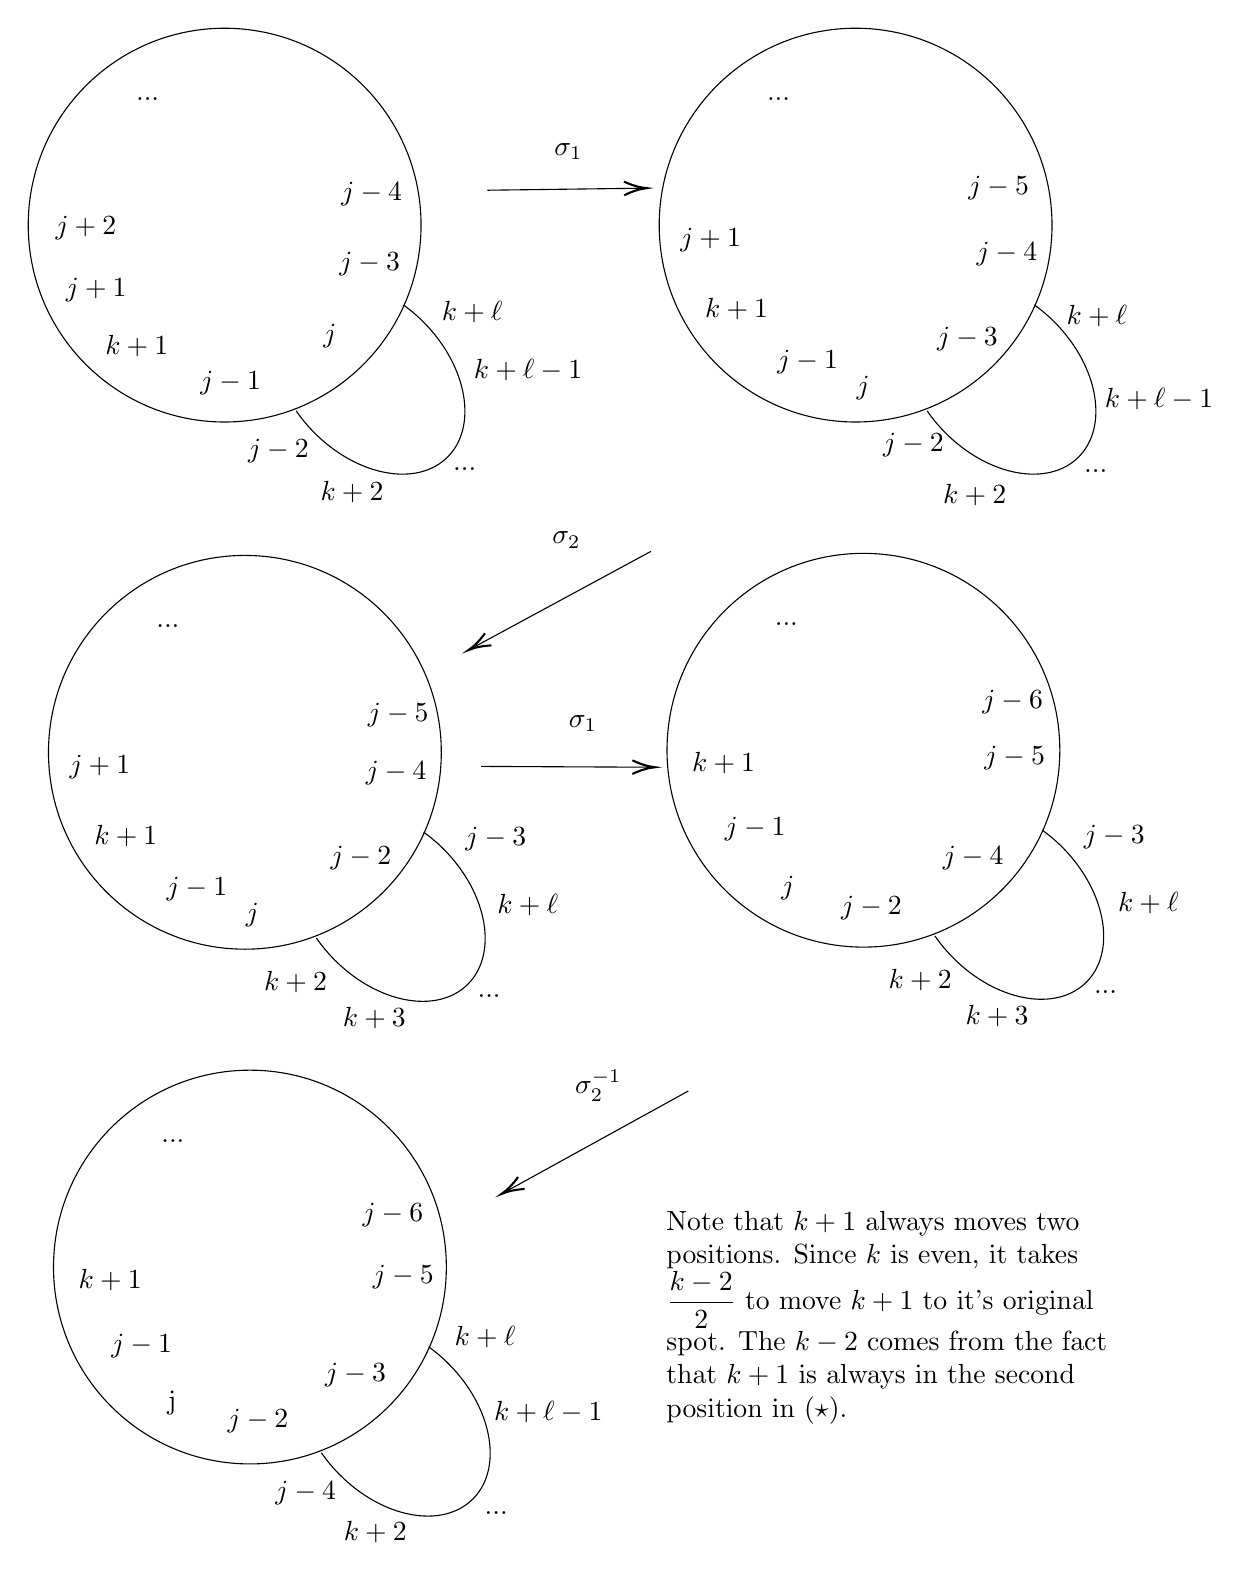
\begin{tikzpicture}[x=0.75pt,y=0.75pt,yscale=-1,xscale=1]
        %uncomment if require: \path (0,796); %set diagram left start at 0, and has height of 796

        %Shape: Ellipse [id:dp11492936941010012] 
        \draw   (19.79,101.81) .. controls (19.79,49.42) and (62.16,6.95) .. (114.42,6.95) .. controls (166.69,6.95) and (209.05,49.42) .. (209.05,101.81) .. controls (209.05,154.2) and (166.69,196.67) .. (114.42,196.67) .. controls (62.16,196.67) and (19.79,154.2) .. (19.79,101.81) -- cycle ;
        %Shape: Arc [id:dp6184922186147035] 
        \draw  [draw opacity=0] (200.55,140.27) .. controls (204.03,142.77) and (207.42,145.65) .. (210.61,148.9) .. controls (231.47,170.14) and (236.44,199.13) .. (221.73,213.66) .. controls (207.01,228.18) and (178.17,222.74) .. (157.31,201.5) .. controls (154.12,198.25) and (151.3,194.81) .. (148.86,191.27) -- (183.96,175.2) -- cycle ; \draw   (200.55,140.27) .. controls (204.03,142.77) and (207.42,145.65) .. (210.61,148.9) .. controls (231.47,170.14) and (236.44,199.13) .. (221.73,213.66) .. controls (207.01,228.18) and (178.17,222.74) .. (157.31,201.5) .. controls (154.12,198.25) and (151.3,194.81) .. (148.86,191.27) ;
        %Straight Lines [id:da0844113158767279] 
        \draw    (241,85) -- (315.8,84.03) ;
        \draw [shift={(317.8,84)}, rotate = 179.25] [color={rgb, 255:red, 0; green, 0; blue, 0 }  ][line width=0.75]    (10.93,-3.29) .. controls (6.95,-1.4) and (3.31,-0.3) .. (0,0) .. controls (3.31,0.3) and (6.95,1.4) .. (10.93,3.29)   ;
        %Shape: Ellipse [id:dp12472713948684278] 
        \draw   (323.79,101.81) .. controls (323.79,49.42) and (366.16,6.95) .. (418.42,6.95) .. controls (470.69,6.95) and (513.05,49.42) .. (513.05,101.81) .. controls (513.05,154.2) and (470.69,196.67) .. (418.42,196.67) .. controls (366.16,196.67) and (323.79,154.2) .. (323.79,101.81) -- cycle ;
        %Shape: Arc [id:dp15059287803772037] 
        \draw  [draw opacity=0] (504.55,140.27) .. controls (508.03,142.77) and (511.42,145.65) .. (514.61,148.9) .. controls (535.47,170.14) and (540.44,199.13) .. (525.73,213.66) .. controls (511.01,228.18) and (482.17,222.74) .. (461.31,201.5) .. controls (458.12,198.25) and (455.3,194.81) .. (452.86,191.27) -- (487.96,175.2) -- cycle ; \draw   (504.55,140.27) .. controls (508.03,142.77) and (511.42,145.65) .. (514.61,148.9) .. controls (535.47,170.14) and (540.44,199.13) .. (525.73,213.66) .. controls (511.01,228.18) and (482.17,222.74) .. (461.31,201.5) .. controls (458.12,198.25) and (455.3,194.81) .. (452.86,191.27) ;
        %Shape: Ellipse [id:dp18020224189504397] 
        \draw   (29.55,355.81) .. controls (29.55,303.42) and (71.91,260.95) .. (124.18,260.95) .. controls (176.44,260.95) and (218.81,303.42) .. (218.81,355.81) .. controls (218.81,408.2) and (176.44,450.67) .. (124.18,450.67) .. controls (71.91,450.67) and (29.55,408.2) .. (29.55,355.81) -- cycle ;
        %Shape: Arc [id:dp24785801004185548] 
        \draw  [draw opacity=0] (210.3,394.27) .. controls (213.79,396.77) and (217.17,399.65) .. (220.37,402.9) .. controls (241.23,424.14) and (246.2,453.13) .. (231.48,467.66) .. controls (216.77,482.18) and (187.93,476.74) .. (167.07,455.5) .. controls (163.88,452.25) and (161.06,448.81) .. (158.62,445.27) -- (193.72,429.2) -- cycle ; \draw   (210.3,394.27) .. controls (213.79,396.77) and (217.17,399.65) .. (220.37,402.9) .. controls (241.23,424.14) and (246.2,453.13) .. (231.48,467.66) .. controls (216.77,482.18) and (187.93,476.74) .. (167.07,455.5) .. controls (163.88,452.25) and (161.06,448.81) .. (158.62,445.27) ;
        %Straight Lines [id:da7880004491491575] 
        \draw    (319.8,259) -- (233.56,305.65) ;
        \draw [shift={(231.8,306.6)}, rotate = 331.59] [color={rgb, 255:red, 0; green, 0; blue, 0 }  ][line width=0.75]    (10.93,-3.29) .. controls (6.95,-1.4) and (3.31,-0.3) .. (0,0) .. controls (3.31,0.3) and (6.95,1.4) .. (10.93,3.29)   ;
        %Shape: Ellipse [id:dp9706999219367343] 
        \draw   (327.55,354.81) .. controls (327.55,302.42) and (369.91,259.95) .. (422.18,259.95) .. controls (474.44,259.95) and (516.81,302.42) .. (516.81,354.81) .. controls (516.81,407.2) and (474.44,449.67) .. (422.18,449.67) .. controls (369.91,449.67) and (327.55,407.2) .. (327.55,354.81) -- cycle ;
        %Shape: Arc [id:dp00727643701865599] 
        \draw  [draw opacity=0] (508.3,393.27) .. controls (511.79,395.77) and (515.17,398.65) .. (518.37,401.9) .. controls (539.23,423.14) and (544.2,452.13) .. (529.48,466.66) .. controls (514.77,481.18) and (485.93,475.74) .. (465.07,454.5) .. controls (461.88,451.25) and (459.06,447.81) .. (456.62,444.27) -- (491.72,428.2) -- cycle ; \draw   (508.3,393.27) .. controls (511.79,395.77) and (515.17,398.65) .. (518.37,401.9) .. controls (539.23,423.14) and (544.2,452.13) .. (529.48,466.66) .. controls (514.77,481.18) and (485.93,475.74) .. (465.07,454.5) .. controls (461.88,451.25) and (459.06,447.81) .. (456.62,444.27) ;
        %Straight Lines [id:da8883833986301954] 
        \draw    (238,362.6) -- (319.8,362.99) ;
        \draw [shift={(321.8,363)}, rotate = 180.27] [color={rgb, 255:red, 0; green, 0; blue, 0 }  ][line width=0.75]    (10.93,-3.29) .. controls (6.95,-1.4) and (3.31,-0.3) .. (0,0) .. controls (3.31,0.3) and (6.95,1.4) .. (10.93,3.29)   ;
        %Shape: Ellipse [id:dp5228009768038788] 
        \draw   (31.97,603.81) .. controls (31.97,551.42) and (74.34,508.95) .. (126.6,508.95) .. controls (178.87,508.95) and (221.24,551.42) .. (221.24,603.81) .. controls (221.24,656.2) and (178.87,698.67) .. (126.6,698.67) .. controls (74.34,698.67) and (31.97,656.2) .. (31.97,603.81) -- cycle ;
        %Shape: Arc [id:dp17179557720291494] 
        \draw  [draw opacity=0] (212.73,642.27) .. controls (216.22,644.77) and (219.6,647.65) .. (222.79,650.9) .. controls (243.65,672.14) and (248.62,701.13) .. (233.91,715.66) .. controls (219.19,730.18) and (190.35,724.74) .. (169.5,703.5) .. controls (166.3,700.25) and (163.48,696.81) .. (161.04,693.27) -- (196.14,677.2) -- cycle ; \draw   (212.73,642.27) .. controls (216.22,644.77) and (219.6,647.65) .. (222.79,650.9) .. controls (243.65,672.14) and (248.62,701.13) .. (233.91,715.66) .. controls (219.19,730.18) and (190.35,724.74) .. (169.5,703.5) .. controls (166.3,700.25) and (163.48,696.81) .. (161.04,693.27) ;
        %Straight Lines [id:da8266227533489909] 
        \draw    (337.8,519) -- (249.55,567.63) ;
        \draw [shift={(247.8,568.6)}, rotate = 331.14] [color={rgb, 255:red, 0; green, 0; blue, 0 }  ][line width=0.75]    (10.93,-3.29) .. controls (6.95,-1.4) and (3.31,-0.3) .. (0,0) .. controls (3.31,0.3) and (6.95,1.4) .. (10.93,3.29)   ;

        % Text Node
        \draw (55.65,153.61) node [anchor=north west][inner sep=0.75pt]   [align=left] {$\displaystyle k+1$};
        % Text Node
        \draw (159.36,224.2) node [anchor=north west][inner sep=0.75pt]   [align=left] {$\displaystyle k+2$};
        % Text Node
        \draw (233.24,165.08) node [anchor=north west][inner sep=0.75pt]   [align=left] {$\displaystyle k+\ell -1$};
        % Text Node
        \draw (223.28,217.28) node [anchor=north west][inner sep=0.75pt]   [align=left] {...};
        % Text Node
        \draw (217.82,137.07) node [anchor=north west][inner sep=0.75pt]   [align=left] {$\displaystyle k+\ell $};
        % Text Node
        \draw (160.68,148.14) node [anchor=north west][inner sep=0.75pt]   [align=left] {$\displaystyle j$};
        % Text Node
        \draw (101.43,170.85) node [anchor=north west][inner sep=0.75pt]   [align=left] {$\displaystyle j-1$};
        % Text Node
        \draw (124.43,203.85) node [anchor=north west][inner sep=0.75pt]   [align=left] {$\displaystyle j-2$};
        % Text Node
        \draw (36.68,126.14) node [anchor=north west][inner sep=0.75pt]   [align=left] {$\displaystyle j+1$};
        % Text Node
        \draw (31.68,96.14) node [anchor=north west][inner sep=0.75pt]   [align=left] {$\displaystyle j+2$};
        % Text Node
        \draw (70.49,38.96) node [anchor=north west][inner sep=0.75pt]   [align=left] {...};
        % Text Node
        \draw (168.43,113.85) node [anchor=north west][inner sep=0.75pt]   [align=left] {$\displaystyle j-3$};
        % Text Node
        \draw (169.43,79.85) node [anchor=north west][inner sep=0.75pt]   [align=left] {$\displaystyle j-4$};
        % Text Node
        \draw (344.65,135.61) node [anchor=north west][inner sep=0.75pt]   [align=left] {$\displaystyle k+1$};
        % Text Node
        \draw (459.36,225.2) node [anchor=north west][inner sep=0.75pt]   [align=left] {$\displaystyle k+2$};
        % Text Node
        \draw (537.24,179.08) node [anchor=north west][inner sep=0.75pt]   [align=left] {$\displaystyle k+\ell -1$};
        % Text Node
        \draw (527.28,218.28) node [anchor=north west][inner sep=0.75pt]   [align=left] {...};
        % Text Node
        \draw (518.82,139.07) node [anchor=north west][inner sep=0.75pt]   [align=left] {$\displaystyle k+\ell $};
        % Text Node
        \draw (417.68,173.14) node [anchor=north west][inner sep=0.75pt]   [align=left] {$\displaystyle j$};
        % Text Node
        \draw (379.43,160.85) node [anchor=north west][inner sep=0.75pt]   [align=left] {$\displaystyle j-1$};
        % Text Node
        \draw (430.43,200.85) node [anchor=north west][inner sep=0.75pt]   [align=left] {$\displaystyle j-2$};
        % Text Node
        \draw (332.68,102.14) node [anchor=north west][inner sep=0.75pt]   [align=left] {$\displaystyle j+1$};
        % Text Node
        \draw (374.49,38.96) node [anchor=north west][inner sep=0.75pt]   [align=left] {...};
        % Text Node
        \draw (456.43,149.85) node [anchor=north west][inner sep=0.75pt]   [align=left] {$\displaystyle j-3$};
        % Text Node
        \draw (475.43,108.85) node [anchor=north west][inner sep=0.75pt]   [align=left] {$\displaystyle j-4$};
        % Text Node
        \draw (272,61.4) node [anchor=north west][inner sep=0.75pt]    {$\sigma _{1}$};
        % Text Node
        \draw (471.43,76.85) node [anchor=north west][inner sep=0.75pt]   [align=left] {$\displaystyle j-5$};
        % Text Node
        \draw (50.4,389.61) node [anchor=north west][inner sep=0.75pt]   [align=left] {$\displaystyle k+1$};
        % Text Node
        \draw (132.12,460.2) node [anchor=north west][inner sep=0.75pt]   [align=left] {$\displaystyle k+2$};
        % Text Node
        \draw (235.04,471.28) node [anchor=north west][inner sep=0.75pt]   [align=left] {...};
        % Text Node
        \draw (244.58,423.07) node [anchor=north west][inner sep=0.75pt]   [align=left] {$\displaystyle k+\ell $};
        % Text Node
        \draw (123.44,427.14) node [anchor=north west][inner sep=0.75pt]   [align=left] {$\displaystyle j$};
        % Text Node
        \draw (85.19,414.85) node [anchor=north west][inner sep=0.75pt]   [align=left] {$\displaystyle j-1$};
        % Text Node
        \draw (164.19,399.85) node [anchor=north west][inner sep=0.75pt]   [align=left] {$\displaystyle j-2$};
        % Text Node
        \draw (38.44,356.14) node [anchor=north west][inner sep=0.75pt]   [align=left] {$\displaystyle j+1$};
        % Text Node
        \draw (80.25,292.96) node [anchor=north west][inner sep=0.75pt]   [align=left] {...};
        % Text Node
        \draw (229.19,390.85) node [anchor=north west][inner sep=0.75pt]   [align=left] {$\displaystyle j-3$};
        % Text Node
        \draw (181.19,358.85) node [anchor=north west][inner sep=0.75pt]   [align=left] {$\displaystyle j-4$};
        % Text Node
        \draw (182.19,330.85) node [anchor=north west][inner sep=0.75pt]   [align=left] {$\displaystyle j-5$};
        % Text Node
        \draw (271,248.4) node [anchor=north west][inner sep=0.75pt]    {$\sigma _{2}$};
        % Text Node
        \draw (170.12,477.2) node [anchor=north west][inner sep=0.75pt]   [align=left] {$\displaystyle k+3$};
        % Text Node
        \draw (338.4,354.61) node [anchor=north west][inner sep=0.75pt]   [align=left] {$\displaystyle k+1$};
        % Text Node
        \draw (433.12,459.2) node [anchor=north west][inner sep=0.75pt]   [align=left] {$\displaystyle k+2$};
        % Text Node
        \draw (532.04,469.28) node [anchor=north west][inner sep=0.75pt]   [align=left] {...};
        % Text Node
        \draw (543.58,422.07) node [anchor=north west][inner sep=0.75pt]   [align=left] {$\displaystyle k+\ell $};
        % Text Node
        \draw (381.44,414.14) node [anchor=north west][inner sep=0.75pt]   [align=left] {$\displaystyle j$};
        % Text Node
        \draw (354.19,385.85) node [anchor=north west][inner sep=0.75pt]   [align=left] {$\displaystyle j-1$};
        % Text Node
        \draw (410.19,423.85) node [anchor=north west][inner sep=0.75pt]   [align=left] {$\displaystyle j-2$};
        % Text Node
        \draw (378.25,291.96) node [anchor=north west][inner sep=0.75pt]   [align=left] {...};
        % Text Node
        \draw (527.19,389.85) node [anchor=north west][inner sep=0.75pt]   [align=left] {$\displaystyle j-3$};
        % Text Node
        \draw (459.19,399.85) node [anchor=north west][inner sep=0.75pt]   [align=left] {$\displaystyle j-4$};
        % Text Node
        \draw (479.19,351.85) node [anchor=north west][inner sep=0.75pt]   [align=left] {$\displaystyle j-5$};
        % Text Node
        \draw (470.12,476.2) node [anchor=north west][inner sep=0.75pt]   [align=left] {$\displaystyle k+3$};
        % Text Node
        \draw (279,337) node [anchor=north west][inner sep=0.75pt]    {$\sigma _{1}$};
        % Text Node
        \draw (478.19,324.85) node [anchor=north west][inner sep=0.75pt]   [align=left] {$\displaystyle j-6$};
        % Text Node
        \draw (42.83,603.61) node [anchor=north west][inner sep=0.75pt]   [align=left] {$\displaystyle k+1$};
        % Text Node
        \draw (170.55,725.2) node [anchor=north west][inner sep=0.75pt]   [align=left] {$\displaystyle k+2$};
        % Text Node
        \draw (238.47,720.28) node [anchor=north west][inner sep=0.75pt]   [align=left] {...};
        % Text Node
        \draw (224,631.07) node [anchor=north west][inner sep=0.75pt]   [align=left] {$\displaystyle k+\ell $};
        % Text Node
        \draw (85.86,662.14) node [anchor=north west][inner sep=0.75pt]   [align=left] {$ $j};
        % Text Node
        \draw (58.61,634.85) node [anchor=north west][inner sep=0.75pt]   [align=left] {$\displaystyle j-1$};
        % Text Node
        \draw (114.61,670.85) node [anchor=north west][inner sep=0.75pt]   [align=left] {$\displaystyle j-2$};
        % Text Node
        \draw (82.67,540.96) node [anchor=north west][inner sep=0.75pt]   [align=left] {...};
        % Text Node
        \draw (161.61,648.85) node [anchor=north west][inner sep=0.75pt]   [align=left] {$\displaystyle j-3$};
        % Text Node
        \draw (137.61,705.85) node [anchor=north west][inner sep=0.75pt]   [align=left] {$\displaystyle j-4$};
        % Text Node
        \draw (184.61,601.85) node [anchor=north west][inner sep=0.75pt]   [align=left] {$\displaystyle j-5$};
        % Text Node
        \draw (179.61,571.85) node [anchor=north west][inner sep=0.75pt]   [align=left] {$\displaystyle j-6$};
        % Text Node
        \draw (282,507.4) node [anchor=north west][inner sep=0.75pt]    {$\sigma _{2}^{-1}$};
        % Text Node
        \draw (243,667.08) node [anchor=north west][inner sep=0.75pt]   [align=left] {$\displaystyle k+\ell -1$};
        % Text Node
        \draw (326,575.6) node [anchor=north west][inner sep=0.75pt]   [align=left] {Note that $\displaystyle k+1$ always moves two\\positions. Since $\displaystyle k$ is even, it takes\\ $\displaystyle \frac{k-2}{2}$ to move $\displaystyle k+1$ to it's original\\spot. The $\displaystyle k-2$ comes from the fact\\that $\displaystyle k+1$ is always in the second\\position in $\displaystyle ( \star )$.};


    \end{tikzpicture}

    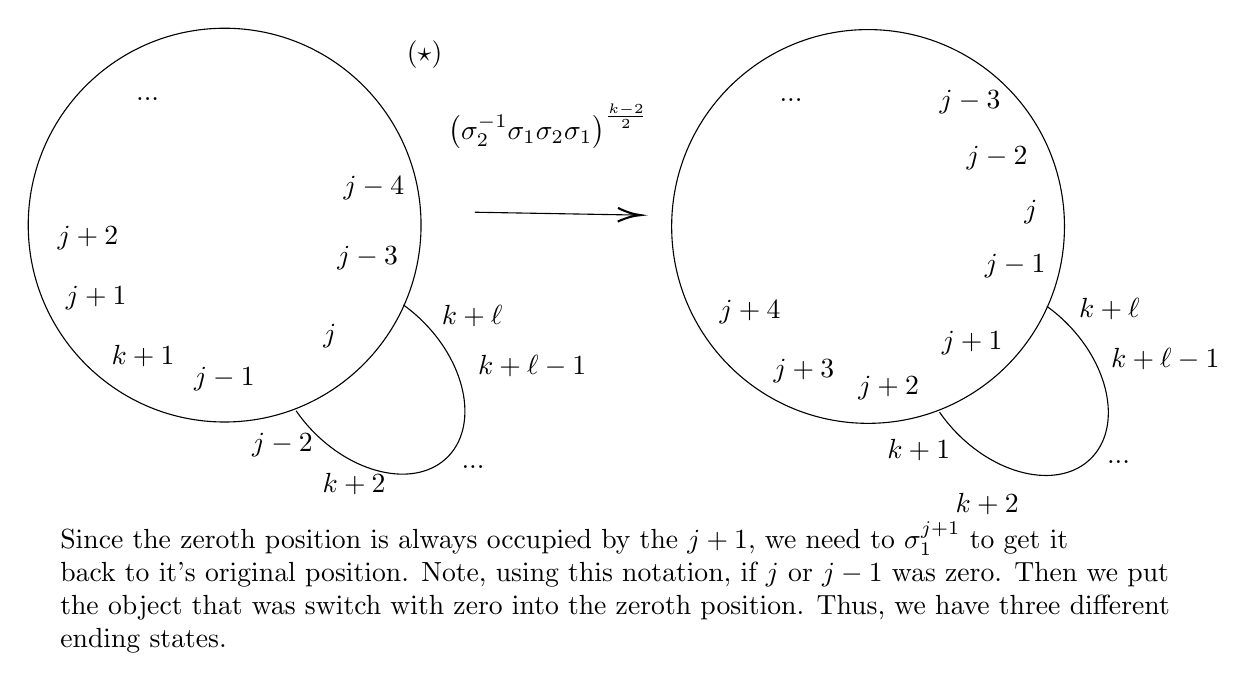
\begin{tikzpicture}[x=0.75pt,y=0.75pt,yscale=-1,xscale=1]
        %uncomment if require: \path (0,365); %set diagram left start at 0, and has height of 365

        %Shape: Ellipse [id:dp14319050725254123] 
        \draw   (24.79,107.21) .. controls (24.79,54.82) and (67.16,12.35) .. (119.42,12.35) .. controls (171.69,12.35) and (214.05,54.82) .. (214.05,107.21) .. controls (214.05,159.6) and (171.69,202.07) .. (119.42,202.07) .. controls (67.16,202.07) and (24.79,159.6) .. (24.79,107.21) -- cycle ;
        %Shape: Arc [id:dp9765775989728762] 
        \draw  [draw opacity=0] (205.55,145.67) .. controls (209.03,148.17) and (212.42,151.05) .. (215.61,154.3) .. controls (236.47,175.54) and (241.44,204.53) .. (226.73,219.06) .. controls (212.01,233.58) and (183.17,228.14) .. (162.31,206.9) .. controls (159.12,203.65) and (156.3,200.21) .. (153.86,196.67) -- (188.96,180.6) -- cycle ; \draw   (205.55,145.67) .. controls (209.03,148.17) and (212.42,151.05) .. (215.61,154.3) .. controls (236.47,175.54) and (241.44,204.53) .. (226.73,219.06) .. controls (212.01,233.58) and (183.17,228.14) .. (162.31,206.9) .. controls (159.12,203.65) and (156.3,200.21) .. (153.86,196.67) ;
        %Straight Lines [id:da8496874476382688] 
        \draw    (240,101) -- (317.8,102.36) ;
        \draw [shift={(319.8,102.4)}, rotate = 181.01] [color={rgb, 255:red, 0; green, 0; blue, 0 }  ][line width=0.75]    (10.93,-3.29) .. controls (6.95,-1.4) and (3.31,-0.3) .. (0,0) .. controls (3.31,0.3) and (6.95,1.4) .. (10.93,3.29)   ;
        %Shape: Ellipse [id:dp09517951855415263] 
        \draw   (334.79,107.86) .. controls (334.79,55.47) and (377.16,13) .. (429.42,13) .. controls (481.69,13) and (524.05,55.47) .. (524.05,107.86) .. controls (524.05,160.25) and (481.69,202.72) .. (429.42,202.72) .. controls (377.16,202.72) and (334.79,160.25) .. (334.79,107.86) -- cycle ;
        %Shape: Arc [id:dp8239879654464959] 
        \draw  [draw opacity=0] (515.55,146.32) .. controls (519.03,148.82) and (522.42,151.7) .. (525.61,154.95) .. controls (546.47,176.19) and (551.44,205.18) .. (536.73,219.7) .. controls (522.01,234.23) and (493.17,228.78) .. (472.31,207.54) .. controls (469.12,204.29) and (466.3,200.86) .. (463.86,197.32) -- (498.96,181.25) -- cycle ; \draw   (515.55,146.32) .. controls (519.03,148.82) and (522.42,151.7) .. (525.61,154.95) .. controls (546.47,176.19) and (551.44,205.18) .. (536.73,219.7) .. controls (522.01,234.23) and (493.17,228.78) .. (472.31,207.54) .. controls (469.12,204.29) and (466.3,200.86) .. (463.86,197.32) ;

        % Text Node
        \draw (63.65,164.01) node [anchor=north west][inner sep=0.75pt]   [align=left] {$\displaystyle k+1$};
        % Text Node
        \draw (165.36,225.6) node [anchor=north west][inner sep=0.75pt]   [align=left] {$\displaystyle k+2$};
        % Text Node
        \draw (240.24,168.48) node [anchor=north west][inner sep=0.75pt]   [align=left] {$\displaystyle k+\ell -1$};
        % Text Node
        \draw (232.28,221.68) node [anchor=north west][inner sep=0.75pt]   [align=left] {...};
        % Text Node
        \draw (222.82,144.47) node [anchor=north west][inner sep=0.75pt]   [align=left] {$\displaystyle k+\ell $};
        % Text Node
        \draw (165.68,153.54) node [anchor=north west][inner sep=0.75pt]   [align=left] {$\displaystyle j$};
        % Text Node
        \draw (103.43,174.25) node [anchor=north west][inner sep=0.75pt]   [align=left] {$\displaystyle j-1$};
        % Text Node
        \draw (131.43,206.25) node [anchor=north west][inner sep=0.75pt]   [align=left] {$\displaystyle j-2$};
        % Text Node
        \draw (41.68,135.54) node [anchor=north west][inner sep=0.75pt]   [align=left] {$\displaystyle j+1$};
        % Text Node
        \draw (37.68,106.54) node [anchor=north west][inner sep=0.75pt]   [align=left] {$\displaystyle j+2$};
        % Text Node
        \draw (75.49,44.36) node [anchor=north west][inner sep=0.75pt]   [align=left] {...};
        % Text Node
        \draw (172.43,116.25) node [anchor=north west][inner sep=0.75pt]   [align=left] {$\displaystyle j-3$};
        % Text Node
        \draw (175.43,82.25) node [anchor=north west][inner sep=0.75pt]   [align=left] {$\displaystyle j-4$};
        % Text Node
        \draw (206,17.35) node [anchor=north west][inner sep=0.75pt]   [align=left] {($\displaystyle \star $)};
        % Text Node
        \draw (382.65,170.65) node [anchor=north west][inner sep=0.75pt]   [align=left] {$\displaystyle j+3$};
        % Text Node
        \draw (470.36,235.25) node [anchor=north west][inner sep=0.75pt]   [align=left] {$\displaystyle k+2$};
        % Text Node
        \draw (545.24,165.13) node [anchor=north west][inner sep=0.75pt]   [align=left] {$\displaystyle k+\ell -1$};
        % Text Node
        \draw (543.28,219.33) node [anchor=north west][inner sep=0.75pt]   [align=left] {...};
        % Text Node
        \draw (529.82,141.11) node [anchor=north west][inner sep=0.75pt]   [align=left] {$\displaystyle k+\ell $};
        % Text Node
        \draw (463.68,157.18) node [anchor=north west][inner sep=0.75pt]   [align=left] {$\displaystyle j+1$};
        % Text Node
        \draw (423.43,178.89) node [anchor=north west][inner sep=0.75pt]   [align=left] {$\displaystyle j+2$};
        % Text Node
        \draw (437.43,208.89) node [anchor=north west][inner sep=0.75pt]   [align=left] {$\displaystyle k+1$};
        % Text Node
        \draw (356.68,142.18) node [anchor=north west][inner sep=0.75pt]   [align=left] {$\displaystyle j+4$};
        % Text Node
        \draw (385.49,45.01) node [anchor=north west][inner sep=0.75pt]   [align=left] {...};
        % Text Node
        \draw (484.43,119.89) node [anchor=north west][inner sep=0.75pt]   [align=left] {$\displaystyle j-1$};
        % Text Node
        \draw (503.43,93.89) node [anchor=north west][inner sep=0.75pt]   [align=left] {$\displaystyle j$};
        % Text Node
        \draw (226,47.4) node [anchor=north west][inner sep=0.75pt]    {$\left( \sigma _{2}^{-1} \sigma _{1} \sigma _{2} \sigma _{1}\right)^{\frac{k-2}{2}}$};
        % Text Node
        \draw (475.68,68.18) node [anchor=north west][inner sep=0.75pt]   [align=left] {$\displaystyle j-2$};
        % Text Node
        \draw (462.68,41.18) node [anchor=north west][inner sep=0.75pt]   [align=left] {$\displaystyle j-3$};
        % Text Node
        \draw (39,249) node [anchor=north west][inner sep=0.75pt]   [align=left] {Since the zeroth position is always occupied by the $\displaystyle j+1$, we need to $\displaystyle \sigma _{1}^{j+1}$ to get it\\back to it's original position. Note, using this notation, if $\displaystyle j$ or $\displaystyle j-1$ was zero. Then we put \\the object that was switch with zero into the zeroth position. Thus, we have three different\\ending states.};


    \end{tikzpicture}

    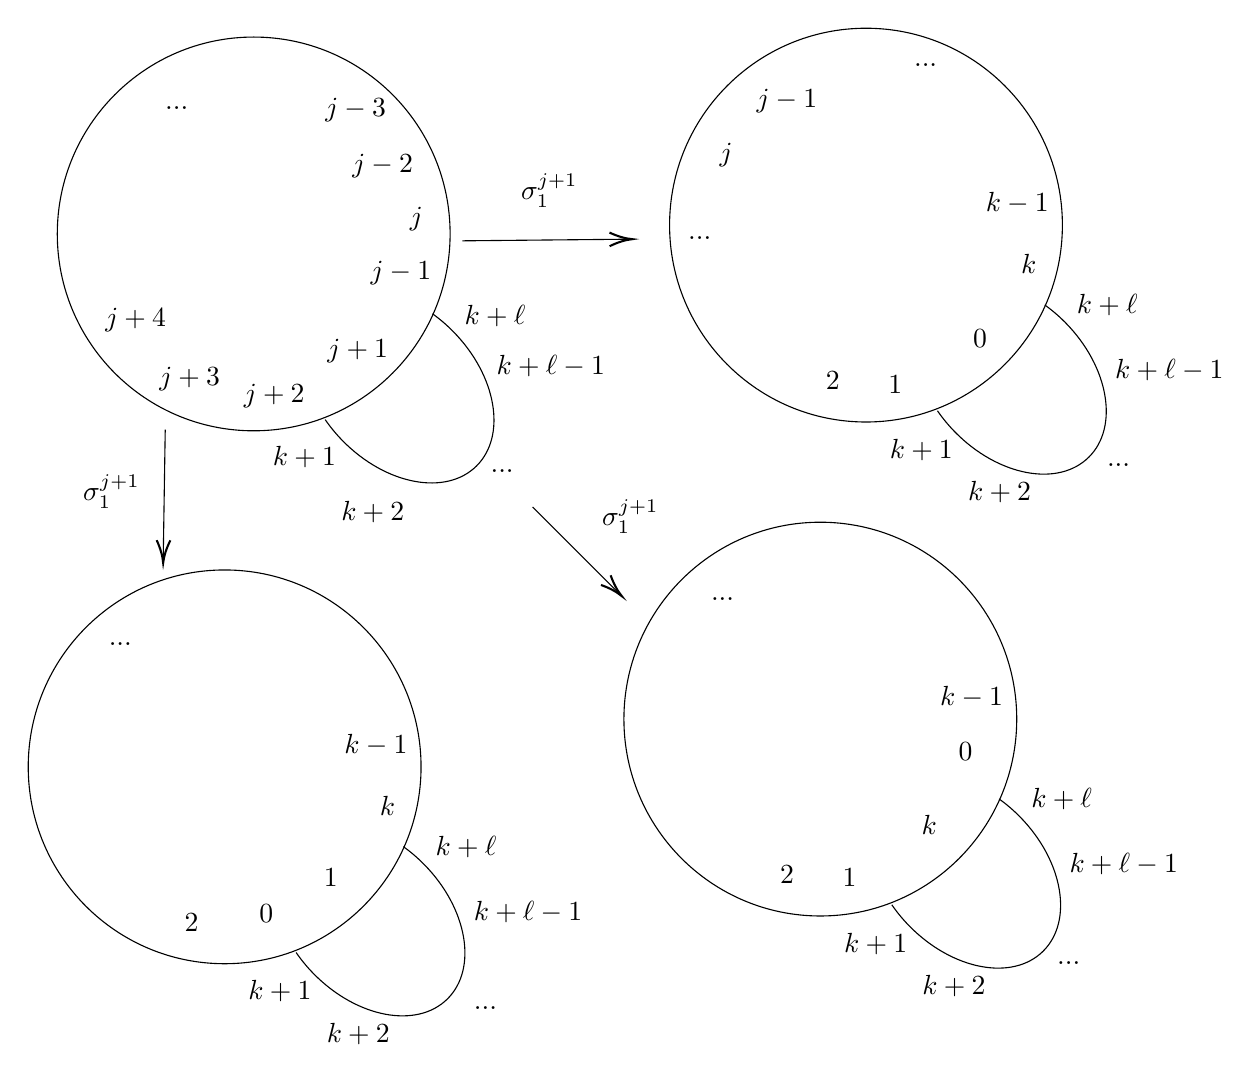
\begin{tikzpicture}[x=0.75pt,y=0.75pt,yscale=-1,xscale=1]
        %uncomment if require: \path (0,636); %set diagram left start at 0, and has height of 636

        %Shape: Ellipse [id:dp7533921208277927] 
        \draw   (47.79,105.85) .. controls (47.79,53.46) and (90.16,11) .. (142.42,11) .. controls (194.69,11) and (237.05,53.46) .. (237.05,105.85) .. controls (237.05,158.24) and (194.69,200.71) .. (142.42,200.71) .. controls (90.16,200.71) and (47.79,158.24) .. (47.79,105.85) -- cycle ;
        %Shape: Arc [id:dp2882722909305362] 
        \draw  [draw opacity=0] (228.55,144.31) .. controls (232.03,146.81) and (235.42,149.69) .. (238.61,152.95) .. controls (259.47,174.18) and (264.44,203.17) .. (249.73,217.7) .. controls (235.01,232.22) and (206.17,226.78) .. (185.31,205.54) .. controls (182.12,202.29) and (179.3,198.85) .. (176.86,195.32) -- (211.96,179.24) -- cycle ; \draw   (228.55,144.31) .. controls (232.03,146.81) and (235.42,149.69) .. (238.61,152.95) .. controls (259.47,174.18) and (264.44,203.17) .. (249.73,217.7) .. controls (235.01,232.22) and (206.17,226.78) .. (185.31,205.54) .. controls (182.12,202.29) and (179.3,198.85) .. (176.86,195.32) ;
        %Straight Lines [id:da7703748103912469] 
        \draw    (243,109.18) -- (322.8,108.4) ;
        \draw [shift={(324.8,108.38)}, rotate = 179.44] [color={rgb, 255:red, 0; green, 0; blue, 0 }  ][line width=0.75]    (10.93,-3.29) .. controls (6.95,-1.4) and (3.31,-0.3) .. (0,0) .. controls (3.31,0.3) and (6.95,1.4) .. (10.93,3.29)   ;
        %Straight Lines [id:da40299510016046347] 
        \draw    (99.8,200.18) -- (98.83,262.38) ;
        \draw [shift={(98.8,264.38)}, rotate = 270.89] [color={rgb, 255:red, 0; green, 0; blue, 0 }  ][line width=0.75]    (10.93,-3.29) .. controls (6.95,-1.4) and (3.31,-0.3) .. (0,0) .. controls (3.31,0.3) and (6.95,1.4) .. (10.93,3.29)   ;
        %Shape: Ellipse [id:dp7504591206154643] 
        \draw   (342.79,101.61) .. controls (342.79,49.22) and (385.16,6.75) .. (437.42,6.75) .. controls (489.69,6.75) and (532.05,49.22) .. (532.05,101.61) .. controls (532.05,154) and (489.69,196.47) .. (437.42,196.47) .. controls (385.16,196.47) and (342.79,154) .. (342.79,101.61) -- cycle ;
        %Shape: Arc [id:dp3607703426088966] 
        \draw  [draw opacity=0] (523.55,140.07) .. controls (527.03,142.57) and (530.42,145.45) .. (533.61,148.7) .. controls (554.47,169.94) and (559.44,198.93) .. (544.73,213.46) .. controls (530.01,227.98) and (501.17,222.54) .. (480.31,201.3) .. controls (477.12,198.05) and (474.3,194.61) .. (471.86,191.07) -- (506.96,175) -- cycle ; \draw   (523.55,140.07) .. controls (527.03,142.57) and (530.42,145.45) .. (533.61,148.7) .. controls (554.47,169.94) and (559.44,198.93) .. (544.73,213.46) .. controls (530.01,227.98) and (501.17,222.54) .. (480.31,201.3) .. controls (477.12,198.05) and (474.3,194.61) .. (471.86,191.07) ;
        %Shape: Ellipse [id:dp00872404803263449] 
        \draw   (33.79,362.61) .. controls (33.79,310.22) and (76.16,267.75) .. (128.42,267.75) .. controls (180.69,267.75) and (223.05,310.22) .. (223.05,362.61) .. controls (223.05,415) and (180.69,457.47) .. (128.42,457.47) .. controls (76.16,457.47) and (33.79,415) .. (33.79,362.61) -- cycle ;
        %Shape: Arc [id:dp5672515404140084] 
        \draw  [draw opacity=0] (214.55,401.07) .. controls (218.03,403.57) and (221.42,406.45) .. (224.61,409.7) .. controls (245.47,430.94) and (250.44,459.93) .. (235.73,474.46) .. controls (221.01,488.98) and (192.17,483.54) .. (171.31,462.3) .. controls (168.12,459.05) and (165.3,455.61) .. (162.86,452.07) -- (197.96,436) -- cycle ; \draw   (214.55,401.07) .. controls (218.03,403.57) and (221.42,406.45) .. (224.61,409.7) .. controls (245.47,430.94) and (250.44,459.93) .. (235.73,474.46) .. controls (221.01,488.98) and (192.17,483.54) .. (171.31,462.3) .. controls (168.12,459.05) and (165.3,455.61) .. (162.86,452.07) ;
        %Shape: Ellipse [id:dp43665981142202503] 
        \draw   (320.79,339.61) .. controls (320.79,287.22) and (363.16,244.75) .. (415.42,244.75) .. controls (467.69,244.75) and (510.05,287.22) .. (510.05,339.61) .. controls (510.05,392) and (467.69,434.47) .. (415.42,434.47) .. controls (363.16,434.47) and (320.79,392) .. (320.79,339.61) -- cycle ;
        %Shape: Arc [id:dp6711321273772175] 
        \draw  [draw opacity=0] (501.55,378.07) .. controls (505.03,380.57) and (508.42,383.45) .. (511.61,386.7) .. controls (532.47,407.94) and (537.44,436.93) .. (522.73,451.46) .. controls (508.01,465.98) and (479.17,460.54) .. (458.31,439.3) .. controls (455.12,436.05) and (452.3,432.61) .. (449.86,429.07) -- (484.96,413) -- cycle ; \draw   (501.55,378.07) .. controls (505.03,380.57) and (508.42,383.45) .. (511.61,386.7) .. controls (532.47,407.94) and (537.44,436.93) .. (522.73,451.46) .. controls (508.01,465.98) and (479.17,460.54) .. (458.31,439.3) .. controls (455.12,436.05) and (452.3,432.61) .. (449.86,429.07) ;
        %Straight Lines [id:da5196639602353341] 
        \draw    (276.8,237.38) -- (318.39,278.96) ;
        \draw [shift={(319.8,280.38)}, rotate = 225] [color={rgb, 255:red, 0; green, 0; blue, 0 }  ][line width=0.75]    (10.93,-3.29) .. controls (6.95,-1.4) and (3.31,-0.3) .. (0,0) .. controls (3.31,0.3) and (6.95,1.4) .. (10.93,3.29)   ;

        % Text Node
        \draw (95.65,168.65) node [anchor=north west][inner sep=0.75pt]   [align=left] {$\displaystyle j+3$};
        % Text Node
        \draw (183.36,233.24) node [anchor=north west][inner sep=0.75pt]   [align=left] {$\displaystyle k+2$};
        % Text Node
        \draw (258.24,163.12) node [anchor=north west][inner sep=0.75pt]   [align=left] {$\displaystyle k+\ell -1$};
        % Text Node
        \draw (255.28,218.33) node [anchor=north west][inner sep=0.75pt]   [align=left] {...};
        % Text Node
        \draw (242.82,139.11) node [anchor=north west][inner sep=0.75pt]   [align=left] {$\displaystyle k+\ell $};
        % Text Node
        \draw (176.68,155.18) node [anchor=north west][inner sep=0.75pt]   [align=left] {$\displaystyle j+1$};
        % Text Node
        \draw (136.43,176.89) node [anchor=north west][inner sep=0.75pt]   [align=left] {$\displaystyle j+2$};
        % Text Node
        \draw (150.43,206.89) node [anchor=north west][inner sep=0.75pt]   [align=left] {$\displaystyle k+1$};
        % Text Node
        \draw (69.68,140.18) node [anchor=north west][inner sep=0.75pt]   [align=left] {$\displaystyle j+4$};
        % Text Node
        \draw (98.49,43.01) node [anchor=north west][inner sep=0.75pt]   [align=left] {...};
        % Text Node
        \draw (197.43,117.89) node [anchor=north west][inner sep=0.75pt]   [align=left] {$\displaystyle j-1$};
        % Text Node
        \draw (216.43,91.89) node [anchor=north west][inner sep=0.75pt]   [align=left] {$\displaystyle j$};
        % Text Node
        \draw (188.68,66.18) node [anchor=north west][inner sep=0.75pt]   [align=left] {$\displaystyle j-2$};
        % Text Node
        \draw (175.68,39.18) node [anchor=north west][inner sep=0.75pt]   [align=left] {$\displaystyle j-3$};
        % Text Node
        \draw (270,75.58) node [anchor=north west][inner sep=0.75pt]    {$\sigma _{1}^{j+1}$};
        % Text Node
        \draw (59,220.58) node [anchor=north west][inner sep=0.75pt]    {$\sigma _{1}^{j+1}$};
        % Text Node
        \draw (487.83,150.58) node [anchor=north west][inner sep=0.75pt]   [align=left] {$\displaystyle 0$};
        % Text Node
        \draw (446.94,172.64) node [anchor=north west][inner sep=0.75pt]   [align=left] {$\displaystyle 1$};
        % Text Node
        \draw (416.82,171.03) node [anchor=north west][inner sep=0.75pt]   [align=left] {$\displaystyle 2$};
        % Text Node
        \draw (350.49,105.76) node [anchor=north west][inner sep=0.75pt]   [align=left] {...};
        % Text Node
        \draw (383.43,34.65) node [anchor=north west][inner sep=0.75pt]   [align=left] {$\displaystyle j-1$};
        % Text Node
        \draw (365.68,60.94) node [anchor=north west][inner sep=0.75pt]   [align=left] {$\displaystyle j$};
        % Text Node
        \draw (459.33,22.38) node [anchor=north west][inner sep=0.75pt]   [align=left] {...};
        % Text Node
        \draw (493.87,84.56) node [anchor=north west][inner sep=0.75pt]   [align=left] {$\displaystyle k-1$};
        % Text Node
        \draw (510.95,114.58) node [anchor=north west][inner sep=0.75pt]   [align=left] {$\displaystyle k$};
        % Text Node
        \draw (447.65,203.41) node [anchor=north west][inner sep=0.75pt]   [align=left] {$\displaystyle k+1$};
        % Text Node
        \draw (485.36,224) node [anchor=north west][inner sep=0.75pt]   [align=left] {$\displaystyle k+2$};
        % Text Node
        \draw (556.24,164.88) node [anchor=north west][inner sep=0.75pt]   [align=left] {$\displaystyle k+\ell -1$};
        % Text Node
        \draw (552.28,215.08) node [anchor=north west][inner sep=0.75pt]   [align=left] {...};
        % Text Node
        \draw (537.82,133.87) node [anchor=north west][inner sep=0.75pt]   [align=left] {$\displaystyle k+\ell $};
        % Text Node
        \draw (143.83,427.58) node [anchor=north west][inner sep=0.75pt]   [align=left] {$\displaystyle 0$};
        % Text Node
        \draw (174.94,410.64) node [anchor=north west][inner sep=0.75pt]   [align=left] {$\displaystyle 1$};
        % Text Node
        \draw (107.82,432.03) node [anchor=north west][inner sep=0.75pt]   [align=left] {$\displaystyle 2$};
        % Text Node
        \draw (71.33,301.38) node [anchor=north west][inner sep=0.75pt]   [align=left] {...};
        % Text Node
        \draw (184.87,345.56) node [anchor=north west][inner sep=0.75pt]   [align=left] {$\displaystyle k-1$};
        % Text Node
        \draw (201.95,375.58) node [anchor=north west][inner sep=0.75pt]   [align=left] {$\displaystyle k$};
        % Text Node
        \draw (138.65,464.41) node [anchor=north west][inner sep=0.75pt]   [align=left] {$\displaystyle k+1$};
        % Text Node
        \draw (176.36,485) node [anchor=north west][inner sep=0.75pt]   [align=left] {$\displaystyle k+2$};
        % Text Node
        \draw (247.24,425.88) node [anchor=north west][inner sep=0.75pt]   [align=left] {$\displaystyle k+\ell -1$};
        % Text Node
        \draw (247.28,477.08) node [anchor=north west][inner sep=0.75pt]   [align=left] {...};
        % Text Node
        \draw (228.82,394.87) node [anchor=north west][inner sep=0.75pt]   [align=left] {$\displaystyle k+\ell $};
        % Text Node
        \draw (480.83,349.58) node [anchor=north west][inner sep=0.75pt]   [align=left] {$\displaystyle 0$};
        % Text Node
        \draw (424.94,410.64) node [anchor=north west][inner sep=0.75pt]   [align=left] {$\displaystyle 1$};
        % Text Node
        \draw (394.82,409.03) node [anchor=north west][inner sep=0.75pt]   [align=left] {$\displaystyle 2$};
        % Text Node
        \draw (361.49,279.76) node [anchor=north west][inner sep=0.75pt]   [align=left] {...};
        % Text Node
        \draw (471.87,322.56) node [anchor=north west][inner sep=0.75pt]   [align=left] {$\displaystyle k-1$};
        % Text Node
        \draw (462.95,384.58) node [anchor=north west][inner sep=0.75pt]   [align=left] {$\displaystyle k$};
        % Text Node
        \draw (425.65,441.41) node [anchor=north west][inner sep=0.75pt]   [align=left] {$\displaystyle k+1$};
        % Text Node
        \draw (463.36,462) node [anchor=north west][inner sep=0.75pt]   [align=left] {$\displaystyle k+2$};
        % Text Node
        \draw (534.24,402.88) node [anchor=north west][inner sep=0.75pt]   [align=left] {$\displaystyle k+\ell -1$};
        % Text Node
        \draw (528.28,455.08) node [anchor=north west][inner sep=0.75pt]   [align=left] {...};
        % Text Node
        \draw (515.82,371.87) node [anchor=north west][inner sep=0.75pt]   [align=left] {$\displaystyle k+\ell $};
        % Text Node
        \draw (309,232.58) node [anchor=north west][inner sep=0.75pt]    {$\sigma _{1}^{j+1}$};


    \end{tikzpicture}

    Let $\psi_j = \sigma_1^{j+1}(\sigma_2^{-1}\sigma_1\sigma_2\sigma_1)^{\frac{k-2}{2}}\sigma_2^{-1}\sigma_1^2\sigma_2\sigma_1^{k+1-j}$ denote the algorithm to transpose the edges $j-1$ and $j$. Then to switch any edges $a$ and $b$, it is the conjugate
    \[ (\psi_{b-1}\psi_{b-2}\dots\psi_{a+2}\psi_{a+1})^{-1}\psi_{b}(\psi_{b-1}\psi_{b-2}\dots\psi_{a+2}\psi_{a+1}). \]
\end{proof}

\begin{theorem}
    Suppose that $G$ is a good 2d-Rubik's shape with distinguished cycles $C_1, C_2, \dots, C_n$. Then adding new vertices defined by \textbf{Definition 6.1} with path $P$ in $G$ having only two vertices results in a new good 2d-Rubik's shape.
\end{theorem}

\begin{proof}
    Base Case: \textbf{Theorem 6.1}.

    Inductive Step: Let $C_i$ be the cycle sharing the edge $\ell$ with the new cycle $C_{n+1}$ and let $\sigma_i$ and $\sigma_{n+1}$ be the cycle in $C_i$ and $C_{n+1}$ respectively. Let $k$ be the size of $C_{n+1}$. Let $\psi_{\ell + 1}$ be the algorithm to swap the edges $\ell$ and $\ell + 1$ in $C_i$.

    We claim that if $\ell \leq j - 1 < j \leq k$ then the product,
    \[ (\sigma_{n+1}\sigma_i\sigma_{n+1}^{k+1-j})^{-1}\psi_{\ell + 1}(\sigma_{n+1}\sigma_i\sigma_{n+1}^{k+1-j}) \]
    will transpose the edges $j-1$ and $j$.

    \textbf{Maybe pics or something here.}

    Then clearly, following the same logic from above, we can switch any edges $a$ and $b$ in $C_{n+1}$ by the conjugate
    \[ (\phi_{b-1}\phi_{b}\dots\phi_{a+2}\phi_{a+1})^{-1}\phi_b(\phi_{b-1}\phi_{b}\dots\phi_{a+2}\phi_{a+1}) \]
    where $\phi_j = (\sigma_{n+1}\sigma_i\sigma_{n+1}^{k+1-j})^{-1}\psi_{\ell + 1}(\sigma_{n+1}\sigma_i\sigma_{n+1}^{k+1-j})$.
\end{proof}

\begin{theorem}
    Suppose that $G$ is a 2d-Rubik's shape with distinguished cycles $C_1, C_2$ and that the length of both $C_1, C_2$ are odd. Then $G$ is not a good 2d-Rubik's shape. \textbf{Do we need the condition $|E(C_1) \cap E(C_2)| = 1$?}
\end{theorem}

\begin{proof}
    Label the edges of $C_1$ by $(0, 1, ..., 2k)$ and the edges of $C_2$ by $(0, 2k + (2\ell - 1), 2k + (2\ell - 2), \dots, k + 2, k+ 1)$, so that if we identify $\sigma_1, \sigma_2$ with the corresponding elements of Sym$(2k + 2\ell)$ then $\sigma_1$ is the cycle $(0, 1, ..., 2k)$ and $\sigma_2$ is the cycle $(0, 2k + (2\ell - 1), 2k + (2\ell - 2), \dots, k + 2, k+ 1)$. Then
    \[ \sigma_1 = (0, 2k - 1, 2k)(0, 2k - 3, 2k - 2)\dots(0, 3, 4)(0, 1, 2), \]
    \[ \sigma_2 = (0, k + 2, k + 1)(0, k + 4, k + 3)\dots(0, 2k + (2\ell - 4), 2k + (2\ell - 3))(0, 2k + (2\ell - 2), 2k + (2\ell - 1)). \]
    Since $\sigma_1$ and $\sigma_2$ are generated by 3-cycles, then $\langle\sigma_1, \sigma_2\rangle$ is generated by the set of 3-cycles. Thus, $\langle\sigma_1, \sigma_2\rangle \subseteq A_{2k + 2\ell}$ and $G$ is not good.
\end{proof}

\end{document}